\documentclass{article}
\usepackage{tikz, comment}
\usepackage{pifont}
\usepackage{fontspec}
\usetikzlibrary{arrows, decorations.markings, decorations.pathreplacing}
\begin{comment}
:Title: Not defined yet
:Tags: area using polar coordinates, polar integral formula ;polar form of a complex number;cardioid;polar coordinates;sohcahtoa
:Prob: 0.5622;0.5576;0.5144;0.4928;0.4574
:Slug: No name yet

Description Here.........
\end{comment}
\begin{document}\centering

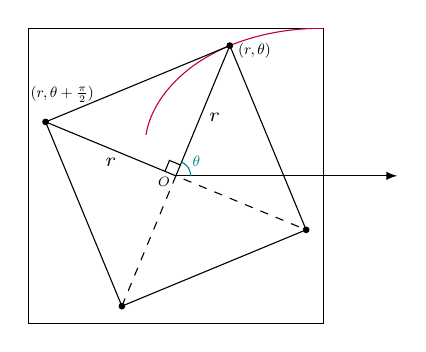
\begin{tikzpicture}[>=latex,xscale=0.375*10/1, yscale=0.375*10/1][font=\sf\small]

%\draw[xstep=1cm,ystep=1cm,color=gray!20] (-2, -2) grid (2, 2);

\draw[->] (0, 0) -- (0.75, 0);
%\draw[] (0, -0.5) -- (0, 0.5);

\clip[draw] (-0.5, -0.5) rectangle (0.5, 0.5);

\draw[purple, samples=100, smooth, domain=pi/4:2.2, variable=\t]
plot ({(1/sqrt(2)*exp(pi/4-\t))*cos(\t r)}, {(1/sqrt(2)*exp(pi/4-\t))*sin(\t r)}); %c=0

\foreach \n in {0,1,2,3}
{
\begin{scope}[rotate around={(\n)*90:({0}, {0})}]

\draw[fill, xscale=1/(10/0.375/0.5), yscale=1/(10/0.375/0.5)] ({(1/sqrt(2)*exp(pi/4-3*pi/8))*cos((3*pi/8) r)*(10/0.375/0.5)}, {(1/sqrt(2)*exp(pi/4-3*pi/8))*sin((3*pi/8) r)*(10/0.375/0.5)}) circle(0.5);

\draw ({(1/sqrt(2)*exp(pi/4-3*pi/8))*cos((3*pi/8) r)}, {(1/sqrt(2)*exp(pi/4-3*pi/8))*sin((3*pi/8) r)})--({(1/sqrt(2)*exp(pi/4-3*pi/8))*cos((3*pi/8+pi/2) r)}, {(1/sqrt(2)*exp(pi/4-3*pi/8))*sin((3*pi/8+pi/2) r)});

\end{scope}
};

\node[right, xshift=1, yshift=-2, scale=0.6] at ({(1/sqrt(2)*exp(pi/4-3*pi/8))*cos((3*pi/8) r)}, {(1/sqrt(2)*exp(pi/4-3*pi/8))*sin((3*pi/8) r)}) {$(r, \theta)$};

\node[above, xshift= 6, yshift= 5, scale=0.6] at ({(1/sqrt(2)*exp(pi/4-3*pi/8))*cos((3*pi/8+pi/2) r)}, {(1/sqrt(2)*exp(pi/4-3*pi/8))*sin((3*pi/8+pi/2) r)}) {$(r, \theta+\frac{\pi}{2})$};

\draw ({(1/sqrt(2)*exp(pi/4-3*pi/8))*cos((3*pi/8+pi/2) r)}, {(1/sqrt(2)*exp(pi/4-3*pi/8))*sin((3*pi/8+pi/2) r)})--(0,0)node[black, below, midway, pos=0.5, yshift=0]{\scriptsize $r$}
--({(1/sqrt(2)*exp(pi/4-3*pi/8))*cos((3*pi/8) r)}, {(1/sqrt(2)*exp(pi/4-3*pi/8))*sin((3*pi/8) r)})node[black, right, midway, pos=0.45, yshift=0]{\scriptsize $r$};

\draw[dashed] ({(1/sqrt(2)*exp(pi/4-3*pi/8))*cos((3*pi/8+2*pi/2) r)}, {(1/sqrt(2)*exp(pi/4-3*pi/8))*sin((3*pi/8+2*pi/2) r)})--(0,0)--({(1/sqrt(2)*exp(pi/4-3*pi/8))*cos((3*pi/8+3*pi/2) r)}, {(1/sqrt(2)*exp(pi/4-3*pi/8))*sin((3*pi/8+3*pi/2) r)});

\draw[rotate around={67.5:({0}, {0})}] ({0+0.04}, 0)--++(0, 0.04)--++(-0.04, 0);
\draw[teal, samples=100, smooth, domain=0:67.5, variable=\t]
plot ({0.05*cos(\t)}, {0.05*sin(\t)});
\node[teal, scale=0.6] at (0.07, 0.05) {$\theta$};

\node[scale=0.7] at ({-0.4/10}, {-0.2/10}) {\scriptsize$O$};

\end{tikzpicture}
\end{document}